\documentclass[jou,a4paper]{apa7}
\usepackage[utf8]{inputenc}
\usepackage[T1]{fontenc}
\usepackage[style=apa, backend=biber]{biblatex}
\usepackage{booktabs}
\usepackage{graphicx}
\usepackage[export]{adjustbox}
\usepackage{listings,multicol}
\usepackage{xcolor}
\usepackage{calc}
\lstset{
  numbers=left,
  firstnumber=1,
  numberfirstline=true,
  basicstyle=\ttfamily\small,
  breaklines=true,
  breakatwhitespace=false,
  frame=single,
  framerule=0.4pt,
  xleftmargin=1em,
  xrightmargin=1em,
  captionpos=b,
  commentstyle=\color{gray},
  keywordstyle=\color{black}
}

\addbibresource{references.bib}

\title{\texttt{bbtkv3}: An Open-Source Suite for Timing Measurement and Analysis with the Black Box ToolKit v3}

\shorttitle{Software for Black Box ToolKit v3}
\leftheader{Pallier}

\authorsnames{Christophe Pallier}
\authorsaffiliations{Cognitive Neuroimaging Unit, CNRS INSERM CEA}

\authornote{\addORCIDlink{Christophe Pallier}{0000-0002-3324-666X} Correspondence should be addressed to C. Pallier,  INSERM, Neurospin, Gif-sur-Yvette, F-91191, France. E-mail: christophe@pallier.org}

\abstract{%
  Experimental psychologists require sub-millisecond accuracy in
  measuring stimulus presentation and participant response times. The
  Black Box ToolKit (BBTK) is a widely used hardware solution for such
  measurements. One limitation is that the software provided with the
  BBTK by the vendor is specific to Windows. We developed a
  cross-platform suite of command line tools and a library designed
  to interface with the BBTK v3. These tools include serial port
  detection, sensor threshold adjustment and automated event
  capture. Additionally, it includes an interactive shell for manual
  device control and a statistical analysis tool that computes event
  durations, jitter, and latencies from captured data. Built in Go,
  the suite is distributed as self-contained binaries for Windows,
  macOS, and Linux. The source code and a library for embedding BBTK
  control in Go applications are available under the GPL-3.0 licence
  at \url{https://github.com/chrplr/bbtkv3}.%
}

\keywords{timing accuracy, stimulus presentation, response time, Black Box ToolKit, open-source software, behavioral research methods}


\begin{document}

\maketitle

\section{Introduction}
\label{sec:introduction}

Precise timing is a cornerstone of experimental psychology. Variations
in stimulus presentation or response recording can introduce noise or
even systematic biases that confound experimental results
\parencite{plant2004}. While modern computers are capable of high
performance, their multi-tasking operating systems and complex
hardware architectures (e.g., display buffering, USB polling) often
introduce unpredictable latencies.


The Black Box ToolKit (BBTK) was developed to address these challenges
by providing an external hardware reference for timing
measurements. It acts as a digital oscilloscope and signal generator,
capable of capturing activity on light and sound sensors, as well as
TTL signals, with sub-millisecond precision. The typical experimental
setup involves three components: a) A \textbf{stimulation device}
(e.g., a computer) running the experimental paradigm; b) The
\textbf{BBTK hardware} with input sensors (photodiodes, microphones)
and TTL inputs/outputs connected to the stimulation device; c) A
\textbf{host computer} (which may be the same as the stimulation
device with our software) driving the BBTK and recording the data (see
Figure~\ref{fig:operation}).

\begin{figure*}[ht]
    \centering
    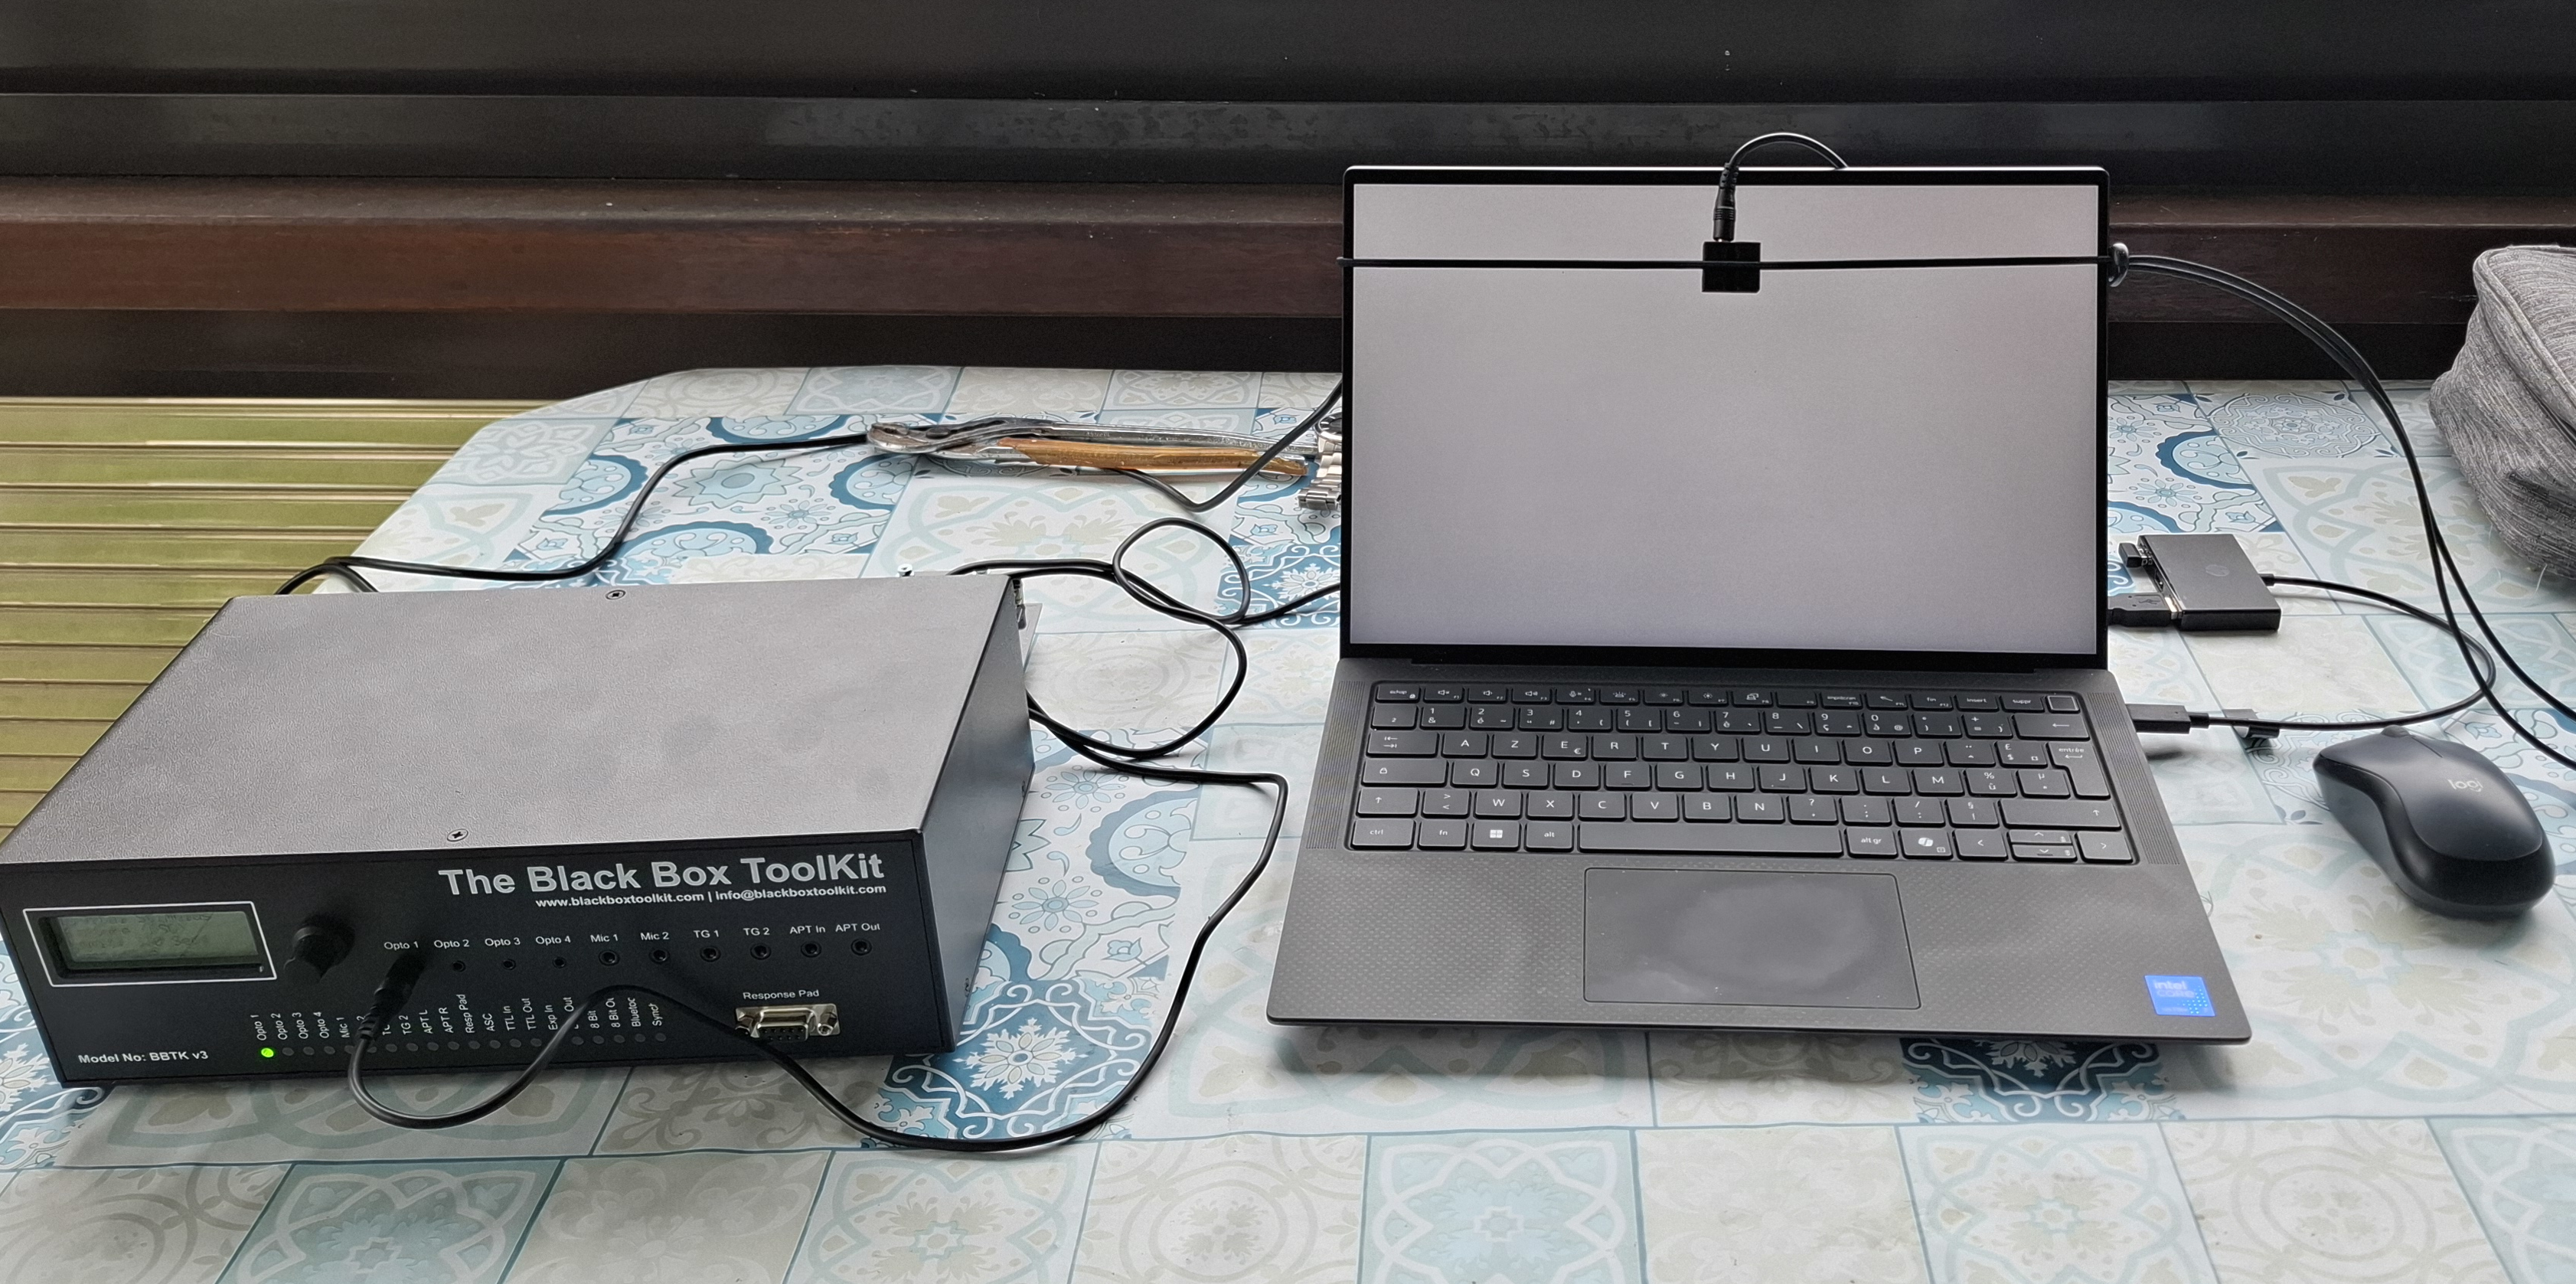
\includegraphics[width=0.8\textwidth]{bbtk-setup.png}
    \caption{Principle of operation: The BBTK acts as an independent
      observer of the stimulation device's outputs. Here an optical
      sensor detects when the illumination of the screen reaches a
      certain threshold. Here, the \texttt{bbtk-capture} program that drives
      the BBTK device during events capture runs on the stimulation
      computer.}
    \label{fig:operation}
\end{figure*}

The BBTK communicates with the host computer via a serial protocol
described in the BBTK API guide \parencite{plant2016}. The
\texttt{bbtkv3} software suite that we developed encapsulates this
protocol into a set of command-line tools and a high-level
library. Designed to be cross-platform (while the vendor's software is
specific to Windows), it is easy to install, and can be integrated
into automated testing workflows. One of its advantages is that the
event capture can run simultaneously on the same computer that runs
the stimulation.


\subsection{Software Suite Components}

The \texttt{bbtkv3} suite consists of several modular CLI tools,
summarized in Table~\ref{tab:tools}. This modularity allows
researchers to use only the components they need or to chain them
together in scripts.

\begin{table*}[ht]
\caption{The \texttt{bbtkv3} toolset}
\label{tab:tools}
\small
\begin{tabular}{@{}lp{0.7\textwidth}@{}}
\toprule
Tool & Description \\
\midrule
\texttt{bbtk-detect-port} & Scans serial ports to locate the connected BBTK. \\
\texttt{bbtk-capture} & Captures events for a specified duration and exports them to CSV and binary formats. \\
\texttt{bbtk-input-check} & Provides a live stream of sensor states for real-time validation. \\
\texttt{bbtk-adjust-thresholds} & Interactive menu for sensor sensitivity calibration. \\
\texttt{bbtk-get-thresholds} & Reads current sensor thresholds from the device. \\
\texttt{bbtk-set-thresholds} & Writes new threshold values to the device. \\
\texttt{bbtk-set-smoothing} & Enables or disables smoothing on individual sensor channels. \\
\texttt{bbtk-event-marking} & Configures the device for real-time event marking. \\
\texttt{bbtk-trigger-response} & Programs the device to answer a trigger on an input line with a delayed pulse on an output line, timed entirely in firmware. \\
\texttt{bbtk-send-command} & Sends raw protocol commands read from standard input and prints the device's replies. \\
\texttt{bbtk-send-break} & Sends the break character to interrupt a running device operation and recover a device left streaming. \\
\texttt{get-serial-port-list} & Lists the serial ports available on the host. \\
\texttt{events-stats} & Performs statistical analysis on captured timing data. \\
\texttt{ibbtk} & An interactive shell providing access to all device functions. \\
\bottomrule
\end{tabular}
\end{table*}

\section{Core Functionality}
\label{sec:functionality}

\subsection{Calibration and Monitoring}

Proper calibration of sensor thresholds is important for reliable
data. The \texttt{bbtk-adjust-thresholds} and
\texttt{bbtk-input-check} tools provide researchers with feedback on
sensor activity, allowing them to set sensitivity levels that
distinguish stimuli from background noise or ambient light.

\subsection{Event Capture and Analysis}

The primary use of \texttt{bbtkv3} is the objective measurement of
latencies. For example, a researcher might want to measure the delay
between a TTL trigger sent by the experimental software and the actual
appearance of a stimulus on the screen (detected by a photodiode).

The \texttt{bbtk-capture} tool automates this process. It can be
launched for a specific duration, during which it records all
transitions on the 12 input lines (4 optical, 2 microphone, 2 TTL, and
4 keypad inputs). All the user has to do is enter the commands shown in
Listing~\ref{lst:capture} below.

\begin{lstlisting}[language=bash, frame=none, numbers=none, caption={Example capture command}, label={lst:capture}, basicstyle=\ttfamily\small]
# Capture for 60 seconds into session1-001*
# (the serial port is located automatically)
bbtk-capture -d 60 session1
# analyse measurements
events-stats session1-001-events.csv
\end{lstlisting}

A practical difficulty is that the stimulus must begin \emph{after} the
device has started recording and end \emph{before} the window closes,
yet the instant at which recording begins cannot be predicted: it
follows a fixed sequence of paced commands and an erasure of the
device's internal memory whose duration depends on whether a full format
or only an erase of the used sectors is required. Waiting a fixed amount
of time is therefore unreliable. The suite offers two ways of
synchronising on that instant instead. The simpler is to let
\texttt{bbtk-capture} start the stimulus itself: everything following a
\texttt{--} separator on its command line is taken as the argument
vector of a child process, launched at the exact moment the device
begins to record, as in Listing~\ref{lst:sync}. No shell is interposed,
so the stimulus keeps its own options unambiguously, and progress
messages move to standard error so that standard output carries only the
stimulus's own. A stimulus that exits with a non-zero status aborts the
capture; one still running when the window closes is terminated, but the
data are downloaded and saved regardless, since the window ran its full
length and the recording is therefore valid.

\begin{lstlisting}[language=bash, frame=none, numbers=none, caption={Running a stimulus inside the capture window}, label={lst:sync}, basicstyle=\ttfamily\small]
bbtk-capture -d 120 session1 -- ./my-stimulus -cycles 1000
\end{lstlisting}

When the stimulus cannot be a child process --- because it is already
running, because it is driven from another language, or because it
executes on a different machine --- \texttt{bbtk-capture} prints the line
\texttt{BBTK-CAPTURE-READY duration=\textit{N}} on its standard output,
on a line of its own, at the instant recording starts. An external
driver launches the capture in the background, blocks until that line
appears, and only then triggers the stimulus. Nothing earlier in the
output identifies that instant, since the messages preceding it are
emitted several seconds before the recording actually begins. A wrapper
can confirm that the binary it is about to drive supports the marker
before touching the device, because \texttt{bbtk-capture -V} advertises
it.

At the end of the event capture, data are downloaded from the BBTK
onto the host PC and saved for further analyses. Among the saved
files, a \texttt{.dat} file contains the raw output of the BBTK and an
\texttt{-events.csv} file consists of a table with four columns:
\texttt{type, onset, duration, durationCorrected}, where \texttt{type}
identifies the sensor (\texttt{Opto1}, \texttt{Mic1}, \texttt{TTLin1},
\ldots), and the remaining columns are expressed in milliseconds
relative to the start of the capture. \texttt{duration} is the value
reported by the device, left unaltered; \texttt{durationCorrected} has
the smoothing tail (see the Limitations section) subtracted on those
channels for which smoothing was actually enabled during the capture,
and repeats \texttt{duration} elsewhere. Onsets need no such correction,
since smoothing extends the trailing edge of a detection rather than
delaying its onset.

\subsection{Statistical Analysis}

This CSV file can easily be imported in a spreadsheet, a Python or R
notebook for inspection. Nevertheless, we provide a command-line tool,
\texttt{events-stats}, which immediately outputs descriptive
statistics and ASCII histograms about the timing data, and also writes
a Markdown and an HTML report containing the same tables together with
log-scale histograms and timeline plots as PNG figures. It computes a)
\textbf{event durations}, that is, the distribution of how long each
sensor remained active; b) \textbf{inter-onset intervals}, the timing
regularity of successive events on a given sensor; c)
\textbf{paired-event onset differences}, the latency between a
reference event (e.g., TTL trigger) and a target event (e.g.,
photodiode detection). Figure~\ref{fig:stats} shows an example of the
output from a simple stimulation program (1 frame on --- 2 frames off)
run on a Raspberry Pi 4.

Two aspects of how these quantities are obtained bear on their
interpretation. First, pairing is by \emph{nearest following} event: for
each occurrence of the reference type, the tool locates the first event
of each other type whose onset is not earlier, and reports the
difference. The pairing is not exclusive, so two reference events
occurring before the sensor responds are both paired with the same
target, and a reference event with no subsequent event of a given type
contributes nothing --- which is why the number of paired observations
can fall short of the number of reference events. Second, the reported
percentiles are computed after an optional outlier filter, enabled by
default, which discards values lying more than 50~ms from the median of
their own series; the threshold is set with \texttt{-detect-outliers}
and disabled by passing zero. Excluded values are always listed in the
output rather than silently dropped, so that the effect of the filter on
any reported figure remains auditable. The filter is treated as
inapplicable, and the series left untouched, when \emph{every} value
would be excluded --- the normal situation for inter-onset intervals,
whose spacing is set by the experimental design and is typically
measured in seconds rather than milliseconds.

  \begin{figure*}
    % The arrow is rendered in a one-character-wide box so that the
    % columns of the ASCII tables stay aligned.
    \begin{lstlisting}[frame=none, numbers=none, basicstyle=\ttfamily\small, literate={→}{{\makebox[\widthof{x}][c]{$\scriptstyle\rightarrow$}}}1]
=== Duration Statistics (ms) ===

Type    N     Min   P5    P25   P50   P75   P95   Max   Range  P95-P05  Mean  SD
----    -     ---   --    ---   ---   ---   ---   ---   -----  -------  ----  --
Opto1   1000  36.5  37.0  37.0  37.2  37.2  37.5  37.8  1.2    0.5      37.2  0.20

  Opto1:
  histogram (10 bins):
  [  36.500,   36.625) ms :     2
  [  36.625,   36.750) ms :     0
  [  36.750,   36.875) ms :    28  **
  [  36.875,   37.000) ms :     0
  [  37.000,   37.125) ms :   283  *************************
  [  37.125,   37.250) ms :     0
  [  37.250,   37.375) ms :   449  ****************************************
  [  37.375,   37.500) ms :     0
  [  37.500,   37.625) ms :   229  ********************
  [  37.625,   37.750) ms :     9

=== Inter-Onset Interval / Jitter Statistics (ms) ===

Type    N    Min   P5    P25   P50   P75   P95   Max   Range  P95-P05  Mean  SD
----    -    ---   --    ---   ---   ---   ---   ---   -----  -------  ----  --
Opto1   999  49.2  49.8  49.8  50.0  50.0  50.2  50.5  1.2    0.5      50.0  0.19

  Opto1:
  histogram (10 bins):
  [  49.250,   49.375) ms :     1
  [  49.375,   49.500) ms :     0
  [  49.500,   49.625) ms :    13  *
  [  49.625,   49.750) ms :     0
  [  49.750,   49.875) ms :   270  **********************
  [  49.875,   50.000) ms :     0
  [  50.000,   50.125) ms :   481  ****************************************
  [  50.125,   50.250) ms :     0
  [  50.250,   50.375) ms :   227  ******************
  [  50.375,   50.500) ms :     7

=== Paired-Event Onset Differences relative to TTLin1 (ms) ===

Type          N     Min   P5    P25   P50   P75   P95   Max   Range  P95-P05  Mean  SD
----          -     ---   --    ---   ---   ---   ---   ---   -----  -------  ----  --
TTLin1→Opto1  1000  31.0  39.0  39.0  39.2  39.2  39.5  39.8  8.8    0.5      39.2  0.32

  TTLin1→Opto1:
  histogram (10 bins):
  [  31.000,   31.875) ms :     1
  [  31.875,   32.750) ms :     0
  [  32.750,   33.625) ms :     0
  [  33.625,   34.500) ms :     0
  [  34.500,   35.375) ms :     0
  [  35.375,   36.250) ms :     0
  [  36.250,   37.125) ms :     0
  [  37.125,   38.000) ms :     0
  [  38.000,   38.875) ms :    22
  [  38.875,   39.750) ms :   977  ****************************************
\end{lstlisting}
\caption{Print out of \texttt{events-stats} from a capture taken while
  the stimulation computer presented 1000 cycles of 1 frame-on, 2
  frames-off. The display monitor refresh rate was fixed at 60Hz. The
  first section show the detected duration of the on-frames; note that
  the BBTK adds 20ms to the duration measures because smoothing was
  set on Opto1). The second section reports on the SOA between
  successive on-frames. The last section display statistics about the
  delay between Opto1 activation and a TTL signal that was sent just
  after the call to display flip. Note the 2-frames delay.}
\label{fig:stats}
\end{figure*}


\subsection{Interactive Usage}

An interactive tool, \texttt{ibbtk}, allows the user to ``manually''
send commands. This is useful for debugging and exploration of the
device's capabilities. It maintains a persistent connection, avoiding
the overhead of re-opening the serial port for each command.

\subsection{Library}

Furthermore, because the entire suite is built upon a modular Go
package, developers can easily integrate BBTK control directly into
their own Go-based experimental or analysis software, e.g.,
\parencite{goxpyrepo}.

\section{Validation}
\label{sec:validation}

A timing tool is only useful if its own measurements can be trusted. We
therefore checked that the suite recovers an interval whose true value
is known by construction. A stimulation program running on a Raspberry
Pi~4 alternated one frame on and two frames off on a display refreshing
at a nominal 60~Hz, so that successive stimulus onsets are separated by
exactly three refresh intervals, i.e. $3 \times 1000/60 = 50.000$~ms.
The program also emitted a TTL pulse immediately after each buffer swap.
A single \texttt{bbtk-capture} run recorded 6000 cycles, and the onset
asynchronies were computed with \texttt{events-stats}.

The measured stimulus onset asynchrony on the photodiode channel had a
median of 50.000~ms, a mean of 49.986~ms and a standard deviation of
0.182~ms, with all 5984 intervals falling between 49.250 and 50.500~ms.
The TTL channel gave a median of 50.000~ms, a mean of 49.985~ms and a
standard deviation of 0.155~ms over 5999 intervals. The suite therefore
recovers the nominal interval exactly at the median, and the residual
0.014~ms departure of the mean corresponds to a refresh rate of
60.017~Hz rather than exactly 60~Hz --- a deviation of 0.03\%, which
illustrates that the resolution of the measurement chain is fine enough
to expose the difference between a monitor's nominal and actual refresh
rate.

% TODO: cross-validation against the vendor's Windows software.
% The check above establishes that the suite recovers a known physical
% interval; it does not establish agreement with the manufacturer's own
% software, since we have no simultaneous recordings from it. Capturing
% the same signal with both and reporting the agreement would close
% this gap, and a reviewer is likely to ask for it.

\section{Limitations}
\label{sec:limitations}

The suite implements the subset of the BBTK serial protocol
\parencite{plant2016} needed to configure the device, to record from it,
and to make it respond: the capture command, the input-check,
event-marking and digital stimulus-response commands, and the commands
that read and write sensor thresholds and the smoothing mask. Output is
supported only in its \emph{reactive} form: \texttt{bbtk-trigger-response}
can raise any of the eight output lines (two TTL outputs, four actuator
closures and two sounders) a programmed delay after a trigger arrives on
an input line, with the delay and the pulse width timed by the device's
own firmware rather than by the host. What the suite does not provide is
autonomous stimulus generation --- there is no way to make the device
emit a sound or a pulse on a schedule of its own, independently of an
input event. Users who need the BBTK to act as a free-running source
must fall back on the vendor's software.

Two further constraints are worth noting. First, the device is driven
over a serial protocol whose command set is documented for the BBTK
v2 \parencite{plant2016}; commands specific to later firmware are not
covered. Second, when smoothing is enabled on an input line, the
durations reported by the device for that line are inflated by
approximately 20~ms, which must be subtracted before interpretation.
\texttt{bbtk-capture} does this automatically in the
\texttt{durationCorrected} column of its output, but the figure is a
measurement made on a single device rather than a constant of the
hardware, and laboratories needing a tighter bound should re-measure it
on their own unit.

\section{Implementation and Availability}
\label{sec:availability}

\texttt{bbtkv3} is written in Go, leveraging the
\texttt{go.bug.st/serial} library for cross-platform serial
communication. By using Go, we are able to provide self-contained,
statically linked binaries that require no runtime environment (like
Python or Java) nor external DLLs.

The software is available for Windows, macOS, and Linux, and Intel and
arm architectures for each operating system. Source code and
pre-compiled binaries are hosted on GitHub
(\url{https://github.com/chrplr/bbtkv3}) under the GNU General Public
Licence v3. Each release is archived on Zenodo: the version described
here is v1.0.13 (\url{https://doi.org/10.5281/zenodo.21620779}), while
\url{https://doi.org/10.5281/zenodo.19551604} always resolves to the
most recent release.

\section*{Author Contributions}

C.P. conceptualized the software, designed the library, and
implemented the tools. Claude Sonnet and Gemini 2.5 were used in the
final phase of the project, to clean some bugs and to develop the
event-stats tool. Consistent with current editorial norms
\parencite{springernature2023}, C.P. takes full responsibility for the
content of the work.

\printbibliography

\end{document}
